% ##################################################################################################################
\section{Cottbus, Germany}
\label{ch:scenarios:cottbus}
\hfill \textbf{Author:} Joschka Bischoff, Dominik Grether
% ##################################################################################################################
\createfigure%
{Cottbus Scenario: Geospatial Location within Germany, Europe}%
{Cottbus Scenario: Geospatial Location within Germany, Europe}%
{\label{fig:scenarios:cottbus_location}}%
{%
  \createsubfigure%
	{Geospatial area of Brandenburg within Germany, Europe (Red); City of Berlin (Yellow)}
	{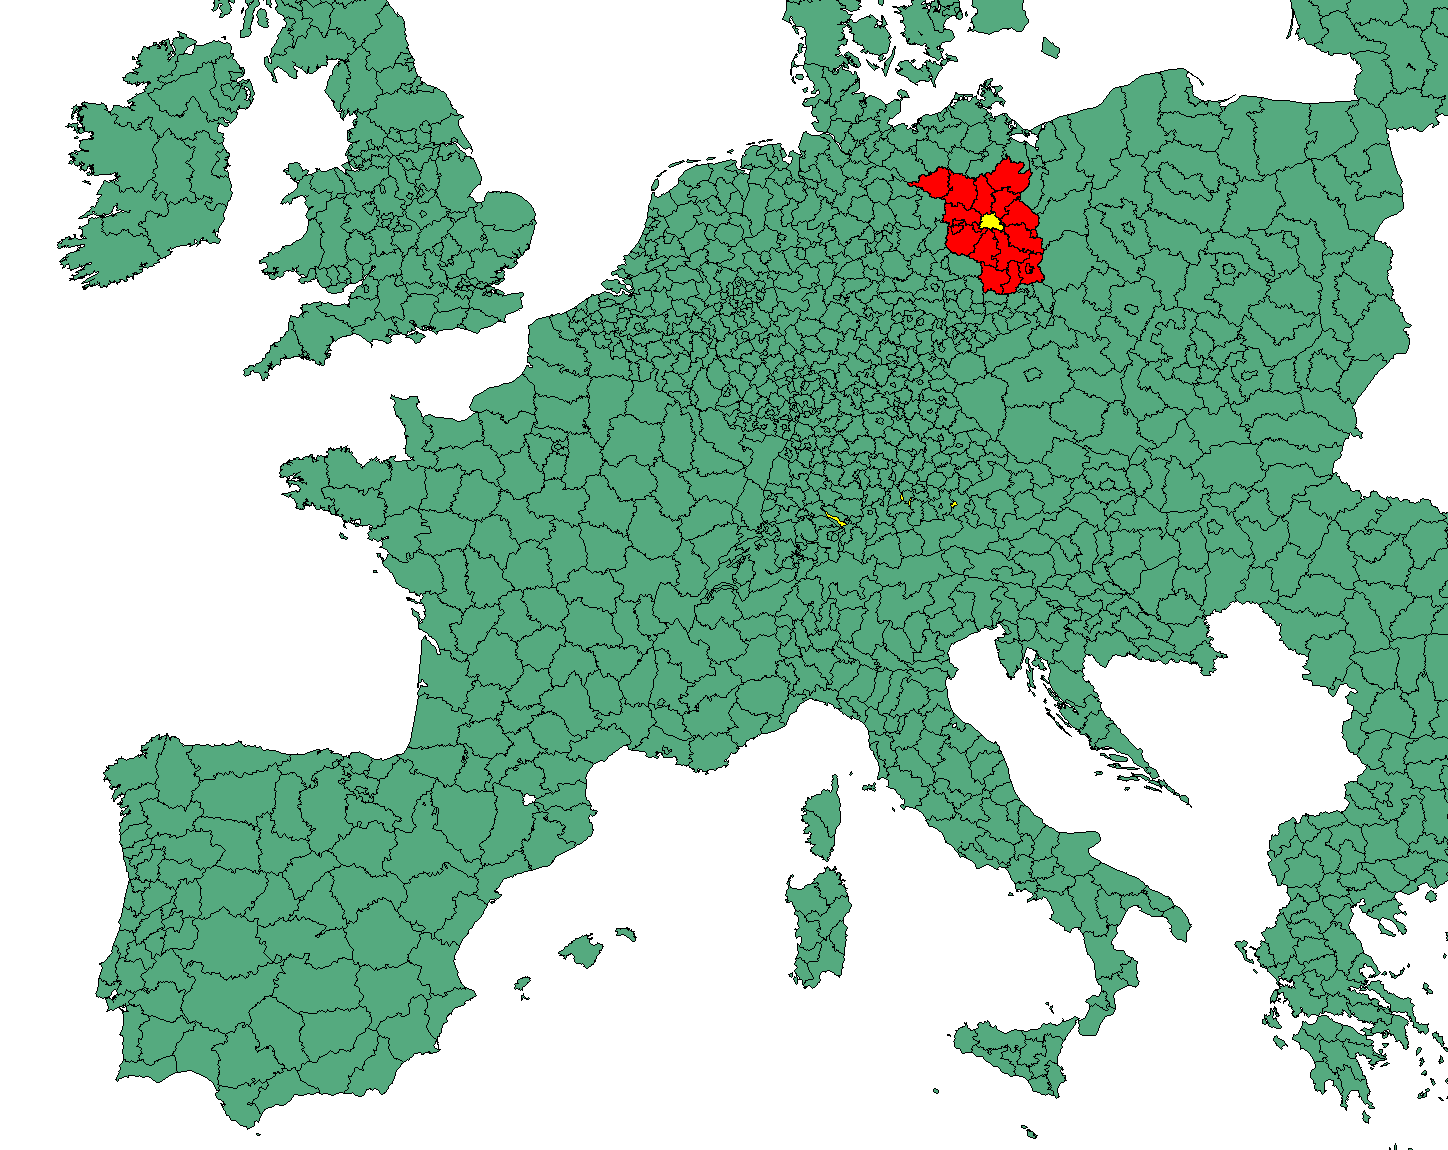
\includegraphics[width=0.49\textwidth]{./using/figures/brandenburg_europe.png}}
	{\label{fig:scenarios:cottbus_brandenburg_europe}}
  \createsubfigure%
	{Geospatial area of Cottbus (Dark Red), within administrative district Spree-Neiße, Brandenburg (Light Red)}
	{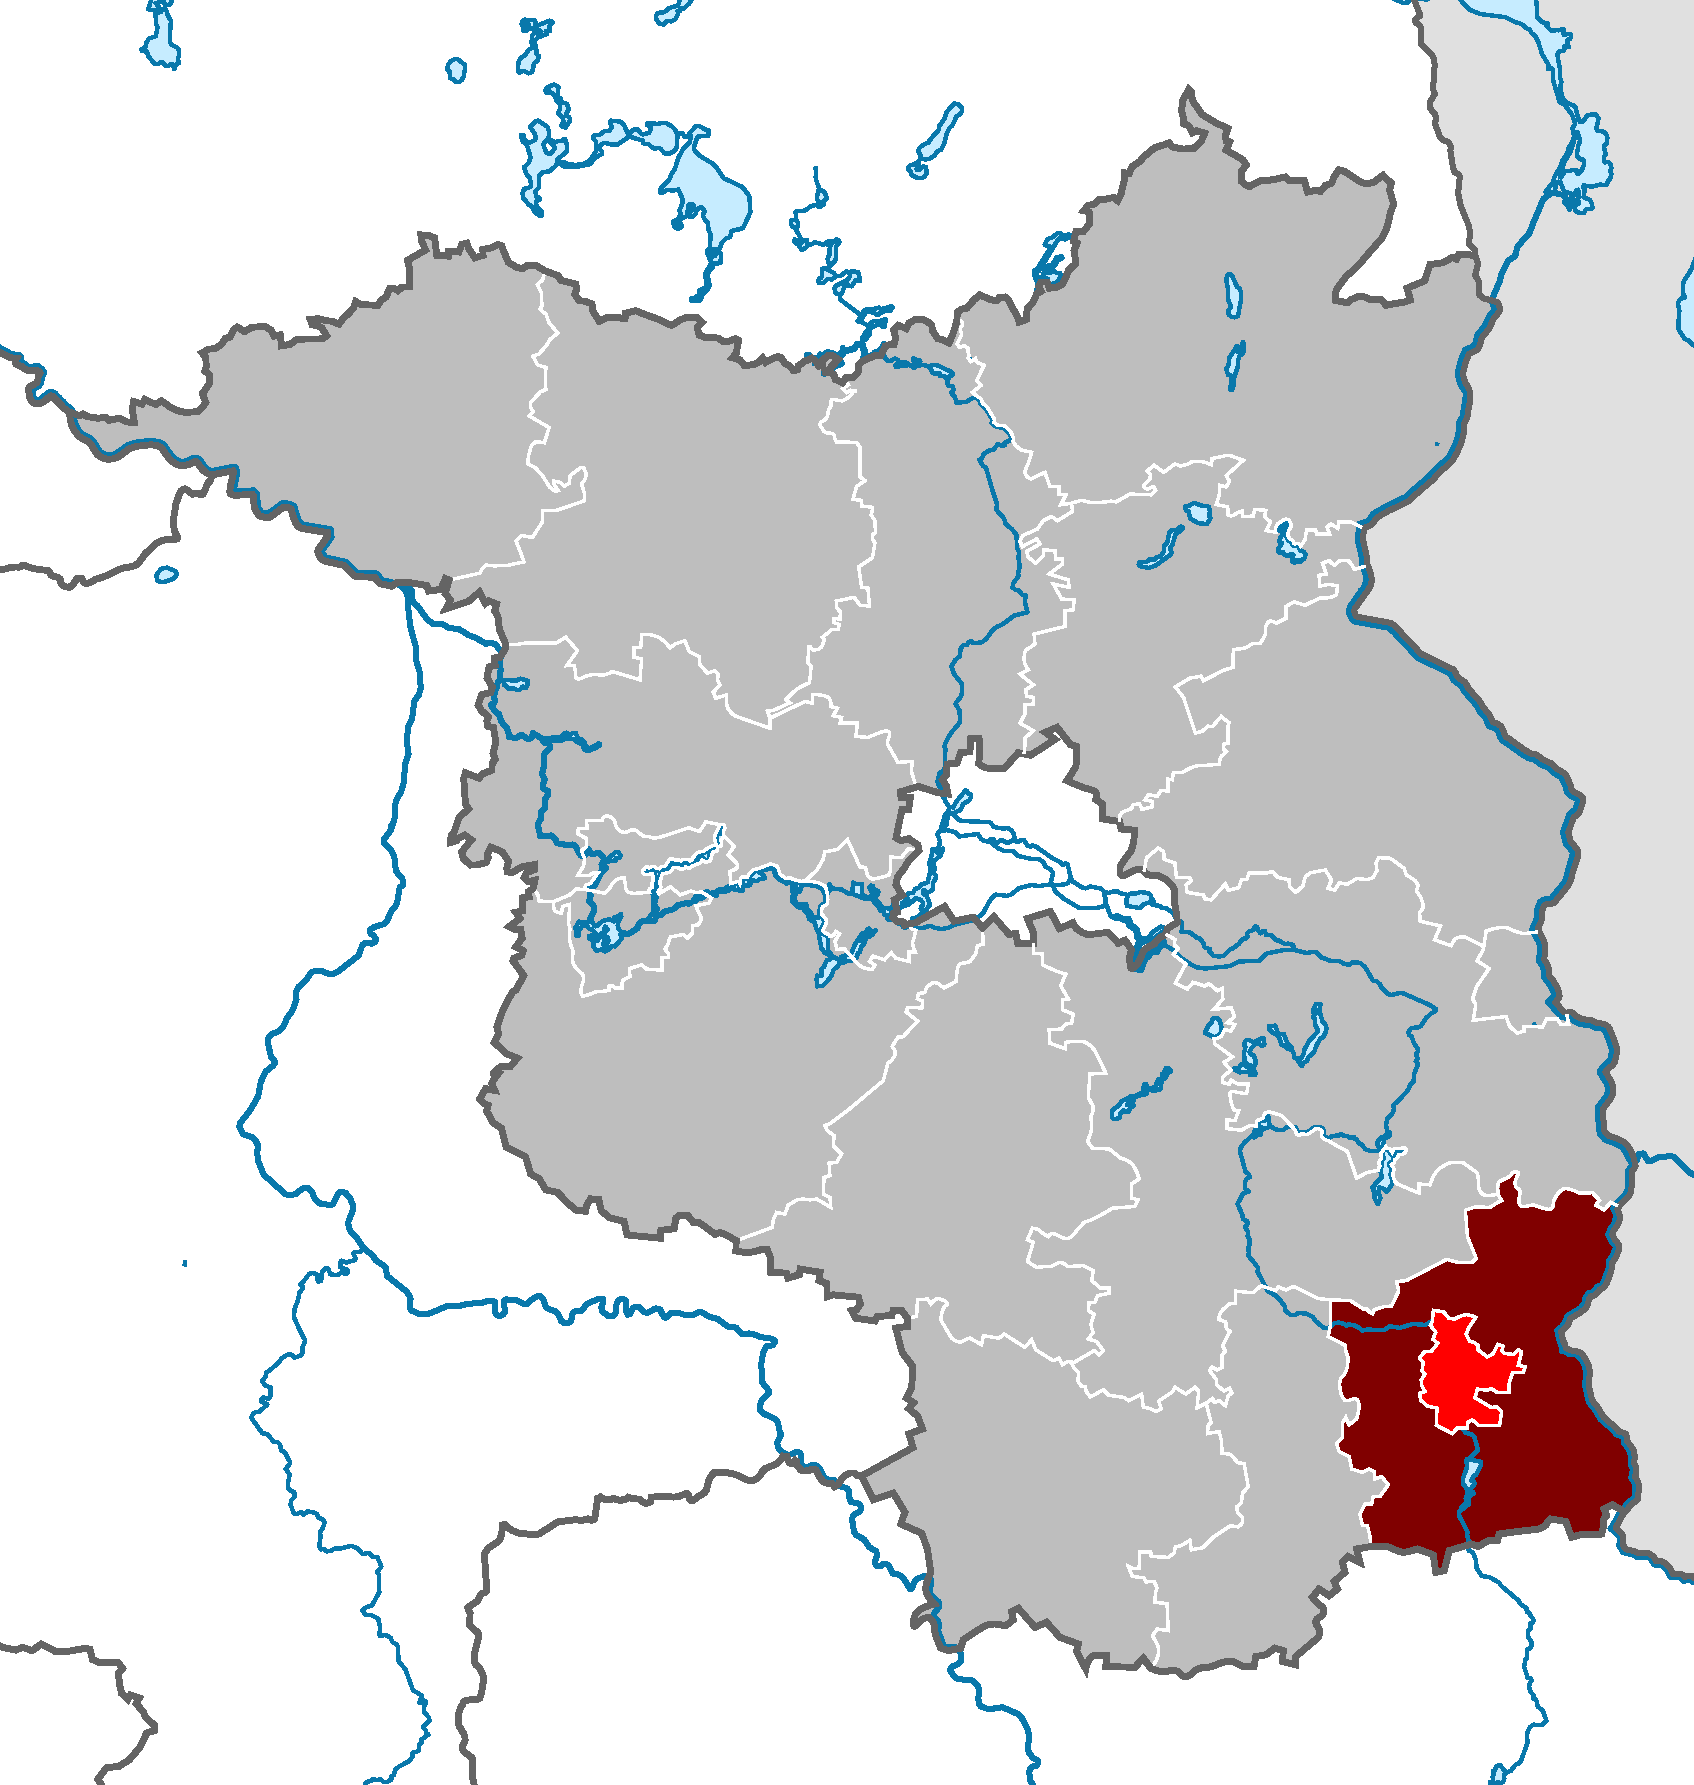
\includegraphics[width=0.49\textwidth]{./using/figures/brandenburg_spree_neise_cottbus.pdf}}
	{\label{fig:scenarios:cottbus_bb}}
}%
{\citet{Grether2014PhD}}

The Cottbus scenario is used for traffic light simulation (see Chapter \ref{ch:signalslanes}). 
It is well described by~\citet[][pp.~87]{Grether_PhDThesis_2014}, this chapter reviews shortly the main points of interest. 
The scenario data is generally available to the public.

The network is taken from openstreetmap data in summer 2010~\citep{Bischoff2010BaSylvia}. 
It covers all streets within the city boundaries and main roads in the surrounding administrative district Spree-Neiße. 
It is designed as a 100 \% sample. 
The population is based on the commuter statistic of the German federal employment agency for both Cottbus and Spree-Neiße~\citep{WiethoelterBogaiCarstensen2010IABPendlerberichtBB}. 
As such, the population has only home-work-home plans that are spread over the usual commuting times, resulting in two peaks. 
Overall, 33'479 agents travelling exclusively by car are included. 
The scenario is overall not very busy, with the area not being known to have bigger congestion issues.


\createfigure%
{Cottbus Scenario: Network and Population}%
{Cottbus Scenario: Network and Population}%
{\label{fig:cottbus_network_population}}%
{%
  \createsubfigure%
	{Cottbus network and municipality borders}
	{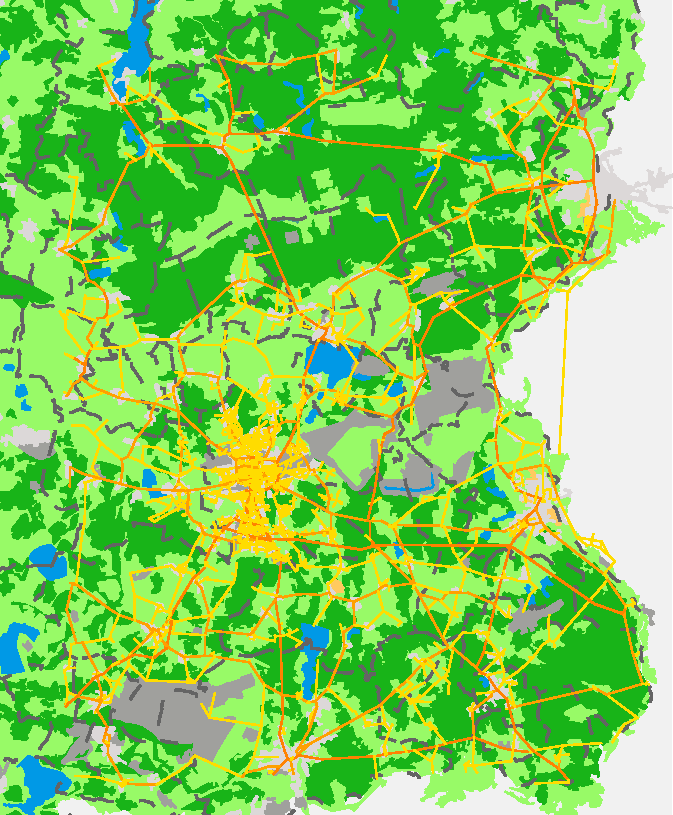
\includegraphics[width=0.49\linewidth]{./using/figures/2013_network_gemeinden_landuse_edit.pdf}}
	{\label{fig:network_municipalities_cottbus_landuse}}
  \createsubfigure%
	{Synthetic population for the Cottbus scenario, geospatial location of home activities}
	{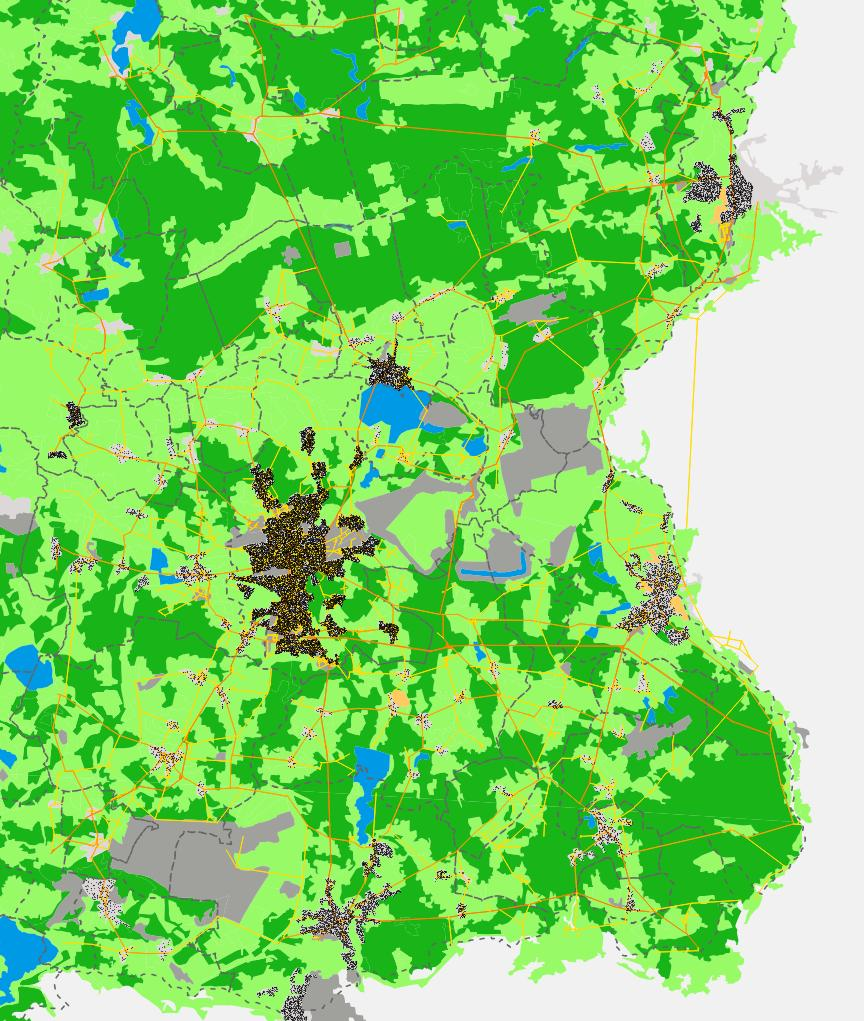
\includegraphics[width=0.49\linewidth]{./using/figures/2013_network_gemeinden_landuse_population_home.jpg}}
	{\label{fig:cottbus_population_home}}
}%
{Source:~\citet{Grether2014PhD}}

Fig.~\ref{fig:network_municipalities_cottbus_landuse} shows the network on top of the 
``Corine Land Cover'' landuse~\citep{CorineLandCover2006Data} provided by European Environmental Agency. 
In green forests and agricultural areas are depicted. 
Area fit for agricultural use covers most of the region.  
Virtual persons in MATSim need a geographic coordinate for their activities. 
If this coordinate is drawn randomly, solely based on municipality boarders, home and work activity locations are uniformly distributed over all the area, i.e., most of them in woods and fields. 
Thus, activity locations are drawn randomly in combination with the landuse data. 
The coordinate has to be in the area of the municipality.  
In case of a home activity, it must be located in 
%(dis-)continuous 
urban fabric areas while in case of a work location, also industrial or commercial areas are allowed. 
The resulting home activity locations are shown in Fig.~\ref{fig:cottbus_population_home}. %, while Fig.~\ref{fig:cottbus_population_work} shows activity locations for work. 

\createfigure%
{Cottbus scenario: Network, area with traffic signals within the city of Cottbus}
{Cottbus scenario: Network, area with traffic signals within the city of Cottbus}
{\label{fig:cottbus_network_signal_locations}}
{%
  \createsubfigure%
	{Location within city of Cottbus}
	{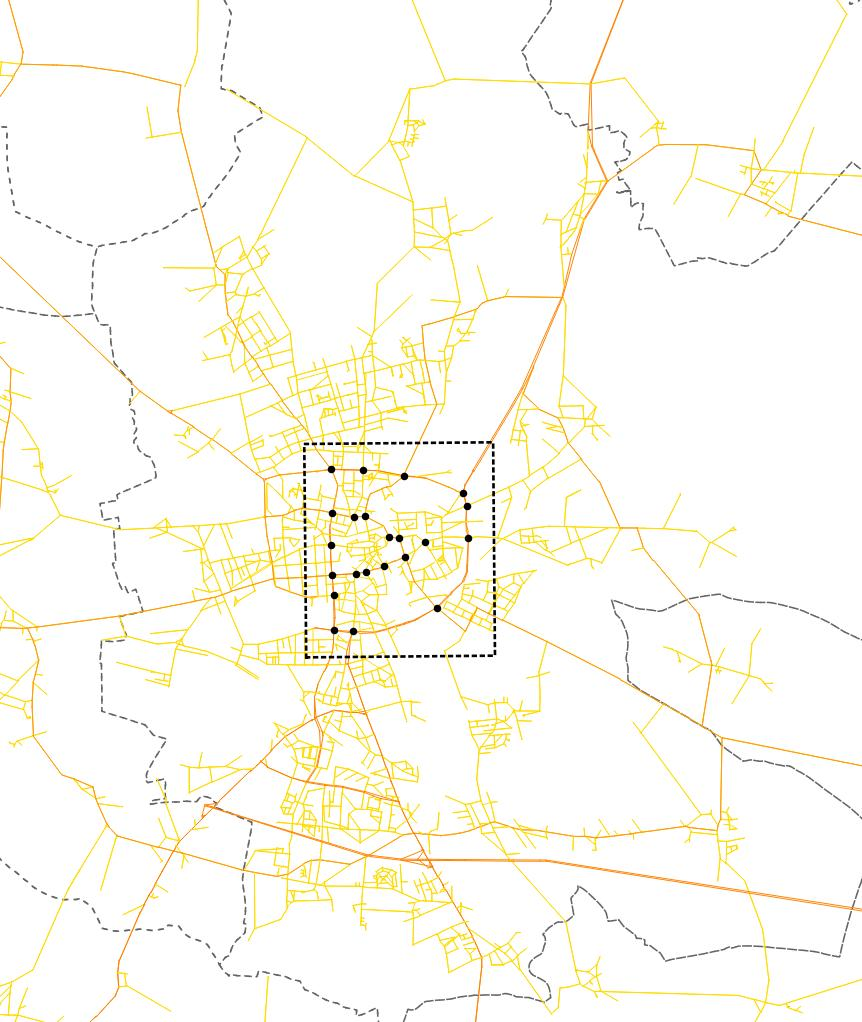
\includegraphics[width=0.49\linewidth]{./using/figures/2013_cottbus_network_signals.jpg}}
	{\label{fig:cottbus_network_signals}}
  \createsubfigure%
	{Signalized area in detail}
	{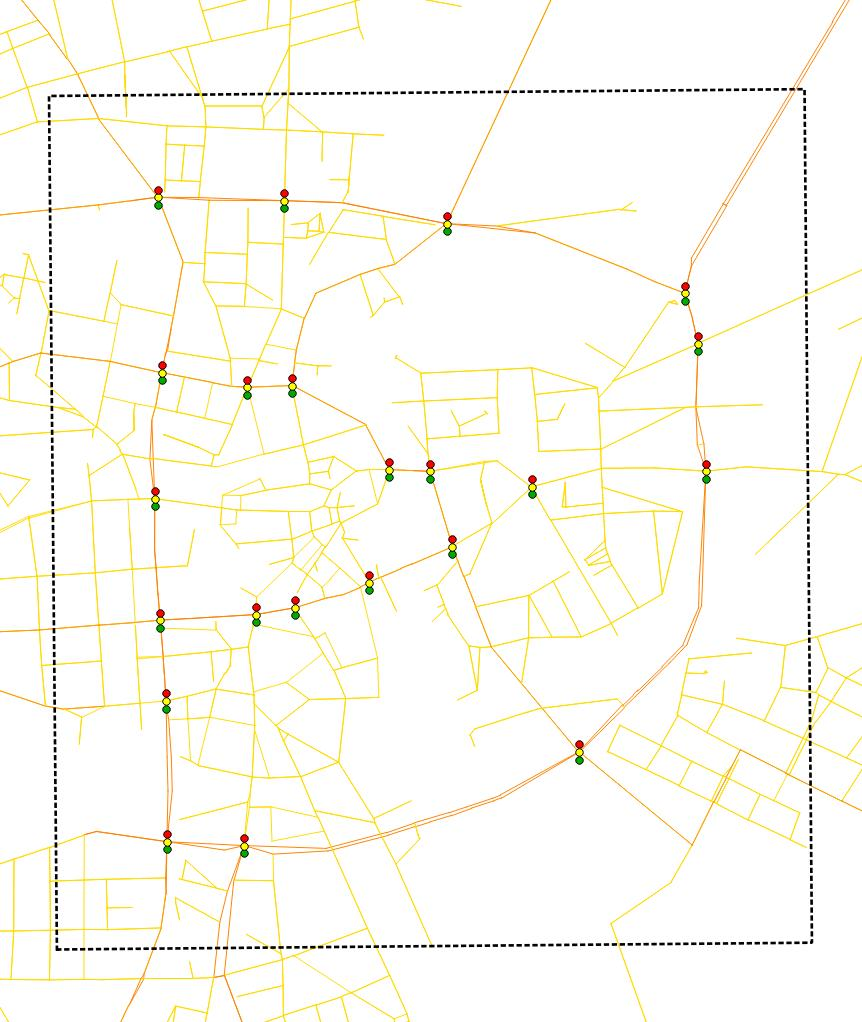
\includegraphics[width=0.49\linewidth]{./using/figures/2013_cottbus_network_signals_zoom.jpg}}
	{\label{fig:cottbus_network_signals_zoom}}
}%
{\citet{Grether2014PhD}}


The scenario contains data for 22 traffic signals within the city centre which are based on the city's signal plans of 2009. 
The junction layout is also modeled in detail.
The fixed-time control data is taken from~\citet{KoehlerStrehler2010SignalDemandOptimization}.  
Due to the higher resolution of the transport network, some of the originally recorded fixed-time control schedules are invalid and removed, data for 22 junctions is available. 
Fig.~\ref{fig:cottbus_network_signal_locations} shows their location on the transport network.  

Public transit, though not part of the original scenario, is available based on the schedules of 2011. The population does, however, not currently use it. 

% ##################################################################################################################

% Andreas Neumann-Mail: frei verfügbar. ÖV vorhanden, 100\% Szenario, das sich mit einigermassen geringem Aufwand rechnen lässt. Grundlage für Dominik G.s Ampelpart
